\documentclass[a4paper,12pt,spanish,final]{epsc_tfc_pfc}

%-----------
% Preamble:
%-----------

\usepackage[spanish,english]{babel}
\usepackage[utf8]{inputenc}
\usepackage{amssymb,amsmath,amsfonts}
\usepackage{array}
\usepackage{listings}
\usepackage{color}

%---------------------------------
% Code snippets style definition:
%---------------------------------

\definecolor{softgray}{RGB}{245,245,245}
\definecolor{softred}{RGB}{222,55,55}
\lstdefinestyle{dnsmasq}{basicstyle=\scriptsize,frame=single,backgroundcolor=\color{softgray},escapeinside={(*@}{@*)}}

%-------------------------------
% Content is about to commence:
%-------------------------------

\begin{document}
\pagestyle{empty}
\selectlanguage{spanish}
\portada{}

%----------
% Resumen:
%----------

\begin{resum}{16cm}
Aquest document conté les pautes del format de presentació del treball o projecte de final de carrera. En tot cas, cal tenir en compte el que estableix la ``Normativa del treball de fi de carrera (TFC) i del projecte de fi de carrera (PFC)'' aprovada per la Comissió Permanent de l'EPSC, especialment l'apartat ``Requeriments del treball''.
\end{resum}
\selectlanguage{english}
\begin{overview}{15cm}
This document contains guidelines for writing your TFC/PFC\@. However, you should also take into consideration the standards established in the document Normativa del treball de fi de carrera (TFC) i del projecte de fi de carrera (PFC), paying special attention to the section Requeriments del treball, as this document has been approved by the EPSC Standing Committee
\end{overview}
\selectlanguage{spanish}

%--------------
% Dedicatoria:
%--------------

\begin{dedicatoria}
Escriure aquí opcionalment la dedicatòria.
\end{dedicatoria}

%-------------------
% Figuras y tablas:
%-------------------

\thispagestyle{empty}
\tableofcontents
\cleardoublepage{}
\thispagestyle{empty}
\listoffigures
\cleardoublepage{}
\thispagestyle{empty}
\listoftables
\cleardoublepage{}
\pagestyle{fancy}

%---------------
% Introducción:
%---------------

\begin{intro}{Introducción}

En este trabajo se presenta una plataforma que pretende dar solución a dos problemáticas de escalabilidad relacionadas con la gestión y la explotación de grandes infraestructuras de computación.

Entendemos por escalabilidad de un sistema a la capacidad del mismo para crecer linealmente y acomodar incrementos de carga computacional. Por otra parte, la escalabilidad de su gestión, viene dada por la capacidad de mantener constante la complejidad de su carga administrativa. Veremos que para dar respuesta a una cuestión, nos centraremos en el ¿Qué? y para la otra en el ¿Cómo?

\textbf{¿Qué?} La plataforma propuesta se cimienta sobre varias tecnologías que interactuan entre ellas. Las más destacables son: Linux (1991), KVM (2007), CoreOS (2013), Docker (2013), Mesos (2011) y Marathon (2013). Las principales virtudes de la solución son su capacidad para acomodar distintos tipos de carga simultáneamente (sin necesidad de realizar un particionado estático) y su simplicidad de escalado mediante la adición de nuevos nodos a base de hardware básico y/o común. En el siguiente esquema simplificado se pueden apreciar las relaciones de orden entre los distintos componentes:\\

\begin{figure}[h]
  \centering
    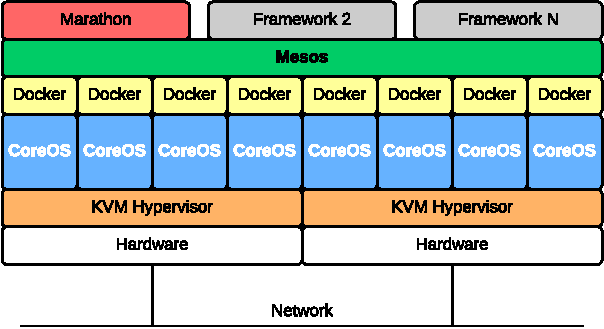
\includegraphics[scale=1]{plataforma}
      \caption{Plataforma}
\end{figure}

En el contexto de este trabajo entendemos por \emph{aprovisionamiento de un sistema} al conjunto de acciones que se deben realizar para disponer de un equipo, ya sea físico o virtual, con un mínimo sistema operativo instanciado y accesible a nivel TCP/IP\@. En el caso de los sistemas físicos, no consideramos las tareas de desempaquetado, ensamblaje, enracado y cableado de los hierros porque se deben realizar en cada centro de datos por un equipo local de operaciones.

Aprovisionar un sistema de forma manual puede suponer entre 20 y 30 minutos. La mayor parte del tiempo se invierte esperando y respondiendo al asistente de instalación. Para ello, además, es necesario tener acceso a la entrada y salida estandar del equipo para visualizar e interactuar con el asistente. Típicamente, con un teclado y un monitor o una redirección de los mismos mediante protocolos tipo \emph{Remote Frame Buffer} o \emph{X Window System Core Protocol}.

Aprovisionar de forma manual es un requisito previo a la automatización ya que nos ayuda a entender las dependencias de orden y a identificar las acciones básicas que se deben realiza para conseguir un sistema funcional.

No se trata de dar mucha inteligencia al sistema de aprovisionamiento sinó de consensar un modelo sencillo y predictible que resulte eficaz en su funcionamiento y simple de mantener. A lo largo de la etapa de aprovisionado intervienen distintas tecnologías que se complementan entre sí.

Una vez aprovisionados, los sistemas sirven de base sobre la que podemos desplegar servicios. Los servicios determinan el rol o la razón de ser de cada equipo. Si bien en la fase de aprovisionado este rol se perfila sutilmente, no es hasta la fase de despliegue, donde se definen con exactitud las funciones de cada equipo y las interrelaciones entre los mismos.

A vista de pájaro el sistema está compuesto por dos grandes bloques funcionales que aglutinan varios servicios; el primer bloque, representado por Cobbler, se encarga de todas las funciones relacionadas con el aprovisionamiento de sistemas. El segundo bloque, representado por Puppet, se encarga de desplegar los servicios y de mantenerlos en el estado deseado.

\begin{figure}[b]
  \centering
    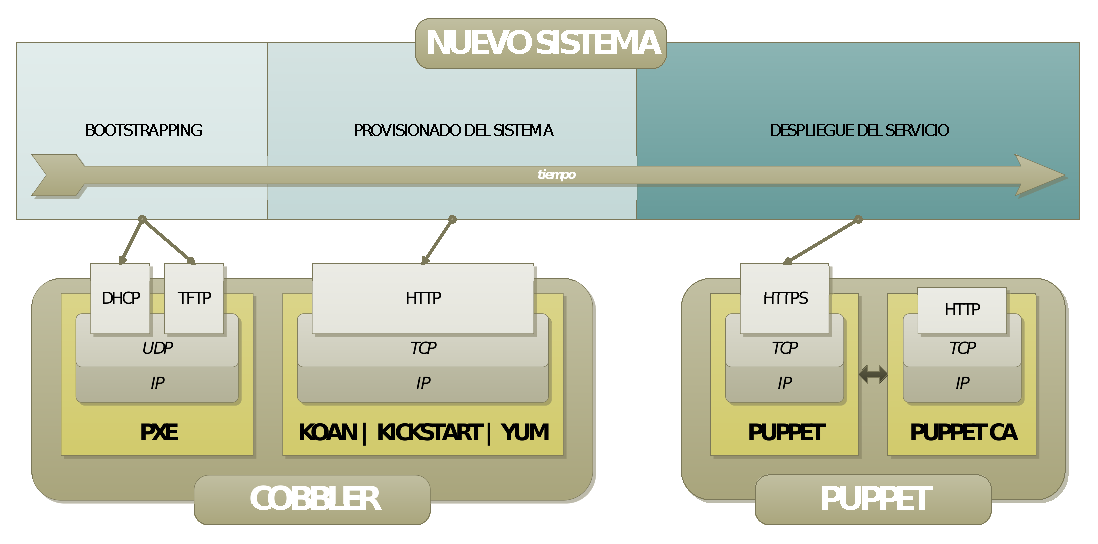
\includegraphics[scale=0.60]{intro}
      \caption{A vista de pájaro}
\end{figure}

\end{intro}

\pagestyle{fancy}

%----------------
% Bootstrapping:
%----------------

\chapter{Bootstrapping}
\section{Pre arranque}
Al pulsar el botón de encendido en un servidor, se inicia el proceso de pre arranque o \emph{`pre boot sequence'}. En el mismo instante en que existe diferencia de potencial, se empiezan a ejecutar una serie de procedimientos basados en hardware que realizan comprobaciones funcionales de la propia electrónica del equipo.

Aquellos componentes electrónicos que dispongan de capacidades \emph{POST} (\emph{Power-On Self Test}), ejecutarán sus rutinas como parte de la secuencia de pre arranque. Si se produjera un error en esta fase, se cancelaría la siguiente fase de arranque y se notificaría el hecho mediante señales acústicas, leds o displays, si el equipo dispone de ellos.

\begin{figure}[h]
  \centering
    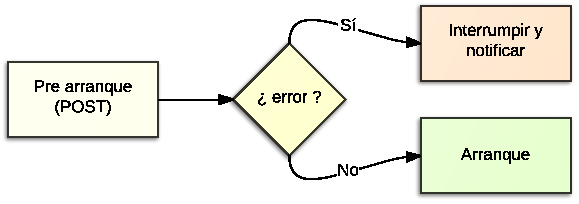
\includegraphics[scale=1]{pre_arranque}
      \caption{Pre arranque}
\end{figure}

\section{Arranque}
Durante el arranque o \emph{`bootstrapping'} se pasa por una serie de fases encadenadas. Cada fase se encarga de preparar el entorno para cargar y ejecutar la siguiente de manera que, en cada fase, se aumentan las funcionalidades y la complejidad del código ejecutado.

La lógica y los datos de las funcionalidades más básicas constituyen el \emph{firmware} del equipo. Éste se encuentra a salvo en direcciones fijas dentro de chips de memoria persistente (\emph{ROM}, \emph{EPROM}, \emph{Flash}) y suele limitarse a proporcionar servicios a una capa superior de software. La vieja y conocida \emph{BIOS} (\emph{Basic Input/Output System}) o la nueva \emph{UEFI} (\emph{Unified Extensible Firmware Interface}), son buenos ejemplos de ello.

Una de las funcionalidades del \emph{firmware} que más nos interesa es la de \emph{`first-stage boot loader'} que se ocupa de localizar, recuperar, cargar en memoria y transferir el control de ejecución al software de arranque o \emph{`bootstrap program'}.

Ejemplos típicos de aplicaciones que encontramos en la categoría de software de arranque son: \emph{LILO}, \emph{GRUB}, \emph{Syslinux}, \emph{PXELinux.0} e incluso podríamos considerar al mismo \emph{kernel} de Linux en esta categoría. Los cuatro primeros se utilizan como \emph{`second-stage boot loaders'} y permiten al usuario gestionar una gran diversidad de opciones de arranque.

\begin{figure}[h]
  \centering
    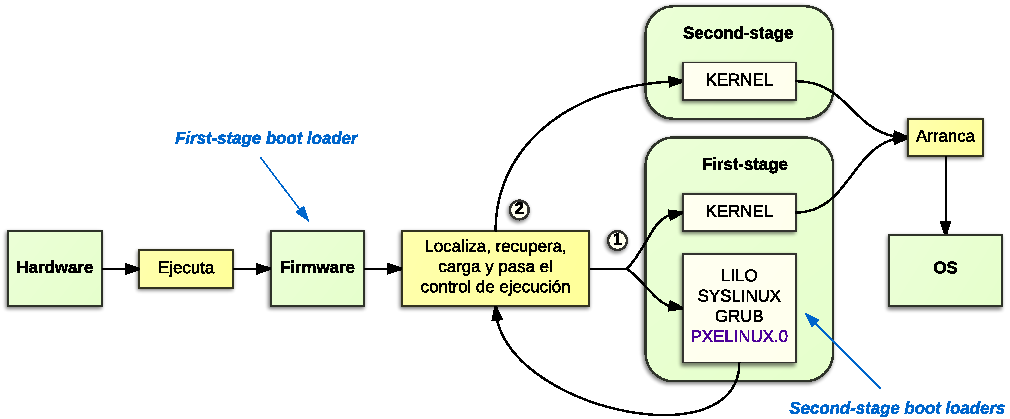
\includegraphics[scale=0.9]{arranque}
      \caption{Arranque}
\end{figure}

\emph{LILO}, \emph{GRUB} y \emph{Syslinux} suelen encontrarse ubicados en el \emph{MBR} (\emph{Master Boot Record}) del dispositivo de arranque, pudiendo ser éste un disco duro, un disquete o un \emph{DVD}. \emph{PXELinux.0} es una variante de \emph{Syslinux} que, a diferencia de los anteriores, se encuentra ubicado en un equipo remoto de la red local.

Puesto que no es lo mismo recuperar el software de arranque desde un \emph{MBR} que desde un equipo remoto, el \emph{firmware} que quiera ejecutar \emph{PXELinux.0}, va a tener que implementar una solución específica. A continuación veremos las tecnologías que lo hacen posible.

\subsection{PXE}
\emph{PXE} (\emph{Pre-Execution Environment}) extiende las funcionalidades del \emph{firmware} dotándolo de capacidades comunicativas gracias a la inclusión de los protocolos \emph{IPv4}, \emph{UDP}, \emph{DHCP} y \emph{TFTP}, estos dos últimos con leves modificaciones. Con estas extensiones, el \emph{firmware} es capaz de localizar, descargar y transferir el control de ejecución al software de arranque \emph{PXELinux.0}, también conocido con el nombre genérico de \emph{NBP} (\emph{Network Bootstrap Program}), que se encuentra ubicado en otro equipo de la red local.

De forma resumida, la mecánica del protocolo \emph{PXE} funciona de la siguiente manera. El cliente inicia el protocolo mediante un broadcast conocido como \emph{DHCPDISCOVER} que contiene unas extensiones (opciones 128 a 135 del \emph{RFC} 4578) que identifican la solicitud como procedente de un equipo que implementa el protocolo \emph{PXE}. En el log del servidor que recive la solicitud podemos ver los siguientes detalles:\\

\begin{lstlisting}[style=dnsmasq]
DHCPDISCOVER(eth1) 00:30:1b:a0:6f:cc
requested options: 1:netmask, 2:time-offset, 3:router, 5, 6:dns-server,
requested options: 11, 12:hostname, 13:boot-file-size, 15:domain-name,
requested options: 16:swap-server, 17:root-path, 18:extension-path,
requested options: 43:vendor-encap, 54:server-identifier, 60:vendor-class,
requested options: 67:bootfile-name, (*@\textcolor{softred}{128}@*), (*@\textcolor{softred}{129}@*), (*@\textcolor{softred}{130}@*), (*@\textcolor{softred}{131}@*), (*@\textcolor{softred}{132}@*),
requested options: (*@\textcolor{softred}{133}@*), (*@\textcolor{softred}{134}@*), (*@\textcolor{softred}{135}@*)
\end{lstlisting}

Asumiendo que en la red existe un servidor \emph{DHCP} o un proxy \emph{DHCP} que también implementa las mismas extensiones del protocolo \emph{DHCP}, el servidor envía al cliente una lista de servidores de arranque (el servidor redirige al cliente) y el nombre del fichero de arranque que el cliente tiene que descargar (\emph{pxelinux.0} en nuestro caso).\\

\begin{lstlisting}[style=dnsmasq]
dnsmasq-dhcp[15]: DHCPOFFER(eth1) 192.168.1.51 00:30:1b:a0:6f:cc
dnsmasq-dhcp[15]: (*@\textcolor{softred}{next server: 192.168.1.2}@*)
dnsmasq-dhcp[15]: sent size:  1 option: 53 message-type  2
dnsmasq-dhcp[15]: option: 54 server-identifier  192.168.1.2
dnsmasq-dhcp[15]: option: 51 lease-time  12h
dnsmasq-dhcp[15]: option: 58 T1  6h
dnsmasq-dhcp[15]: option: 59 T2  10h30m
dnsmasq-dhcp[15]: option: 67 (*@\textcolor{softred}{bootfile-name  pxelinux.0}@*)
dnsmasq-dhcp[15]: option:  1 netmask  255.255.255.0
dnsmasq-dhcp[15]: option: 28 broadcast  192.168.1.255
dnsmasq-dhcp[15]: option:  3 router  192.168.1.1
dnsmasq-dhcp[15]: option:  6 dns-server  192.168.1.2
dnsmasq-dhcp[15]: available DHCP range: 192.168.1.50 -- 192.168.1.150
\end{lstlisting}

A continuación, el cliente utiliza \emph{TFTP} para descargar el \emph{NBP} de uno de los servidores de arranque. Finalmente, el \emph{firmware} del cliente transfiere el control de ejecución a la imagen descargada.\\

\begin{lstlisting}[style=dnsmasq]
dnsmasq-tftp[15]: (*@\textcolor{softred}{sent /tftpboot/pxelinux.0 to 192.168.1.51}@*)
\end{lstlisting}

\subsubsection{PXELinux.0}
\emph{PXELinux.0} actua como \emph{`Second Stage Boot Loader'} permitiendo localizar, descargar y pasar el control de ejecución al \emph{kernel} de Linux y a su correspondiente \emph{initramfs} (\emph{Initial RAM File System}). \emph{PXELinux.0} comunica al \emph{kernel} la dirección de memoria en la que ha cargado el \emph{initramfs}. La ejecución del \emph{kernel} puede ser parametrizada mediante un fichero de configuración que además, permite definir menús interactivos. El primer fichero que \emph{PXELinux.0} intenta descargar del servidor \emph{TFTP} es por tanto, su propio fichero de configuración.

Cada cliente puede disponer de su propio fichero de configuración. El nombre del fichero de cada equipo queda determinado por su direcin \emph{MAC} o la conversión a hexadecimal de su direción \emph{IP}. Si no existe fichero alguno con ese nombre, se procede a eliminar un dígito hexadecimal del final del nombre y se repite la búsqueda sucesivamente tal y como se muestra en la siguiente captura:\\

\begin{lstlisting}[style=dnsmasq]
dnsmasq-tftp[15]: file /tftpboot/pxelinux.cfg/01-00-30-1b-a0-6f-cc not found
dnsmasq-tftp[15]: file /tftpboot/pxelinux.cfg/C0A80233 not found
dnsmasq-tftp[15]: file /tftpboot/pxelinux.cfg/C0A8023 not found
dnsmasq-tftp[15]: file /tftpboot/pxelinux.cfg/C0A802 not found
dnsmasq-tftp[15]: file /tftpboot/pxelinux.cfg/C0A80 not found
dnsmasq-tftp[15]: file /tftpboot/pxelinux.cfg/C0A8 not found
dnsmasq-tftp[15]: file /tftpboot/pxelinux.cfg/C0A not found
dnsmasq-tftp[15]: file /tftpboot/pxelinux.cfg/C0 not found
dnsmasq-tftp[15]: file /tftpboot/pxelinux.cfg/C not found
dnsmasq-tftp[15]: (*@\textcolor{softred}{sent /tftpboot/pxelinux.cfg/default to 192.168.1.51}@*)
dnsmasq-tftp[15]: (*@\textcolor{softred}{sent /tftpboot/menu.c32 to 192.168.1.51}@*)
\end{lstlisting}

Si finalmente no se encuentra ninguna configuración, se utilizará el fichero por defecto llamado \emph{`default'}. Para la realización de este proyecto se ha definido que todos los equipos físicos dispongan de configuración específica y que las máquinas virtuales usen la configuración por defecto. Por ejemplo, al equipo físico que realizará funciones de hipervisor se le aplica la siguiente configuración:\\

\begin{lstlisting}[style=dnsmasq]
DEFAULT menu.c32
PROMPT 0
TIMEOUT 100
ONTIMEOUT local

MENU TITLE Main Menu

LABEL local
  MENU LABEL Boot local hard drive
  LOCALBOOT 0

LABEL install
  MENU LABEL Unattended CentOS 7 installation
  KERNEL images/centos/7/x86_64/vmlinuz
  IPAPPEND 2
  APPEND initrd=images/centos/7/x86_64/initrd.img rd.driver.pre=loop
         inst.repo=http://repo01.demo.lan/centos/7/os/x86_64/
         inst.ks=nfs:boot01.demo.lan:/kickstart/kvm.ks
         inst.geoloc=0 inst.text
\end{lstlisting}

Tras descargar el fichero de configuración de \emph{PXELinux.0} se procede a su interpretación. La primera línea (\emph{DEFAULT menu.c32}) provoca la descarga mediante \emph{TFTP} de otro binario cuya única función es presentar un menú interactivo en la consola del sistema. El resto del fichero contiene la configuración de dicho menú. Cada elemento seleccionable contiene la información necesaria para localizar a una pareja de \emph{kernel} y \emph{initramfs} así como los parámetros adicionales que se le quieran entregar al \emph{kernel} en el momento de su ejecución.

El aspecto del menú que nos presenta \emph{menu.c32} es el siguiente:\\

\begin{lstlisting}[style=dnsmasq]
                   +----------------------------------------------------------+
                   |                        Main Menu                         |
                   +----------------------------------------------------------+
                   | Boot local hard drive                                    |
                   | Unattended CentOS 7 installation                         |
                   |                                                          |
                   |                                                          |
                   |                                                          |
                   |                                                          |
                   |                                                          |
                   |                                                          |
                   |                                                          |
                   |                                                          |
                   |                                                          |
                   |                                                          |
                   +----------------------------------------------------------+

                                     Press [Tab] to edit options

                                    Automatic boot in 7 seconds...
\end{lstlisting}

Si pulsamos \emph{[Tab]} sobre la opción \emph{`Unattended CentOS 7 installation'} podremos editar la línea del comando que se ejecuta al seleccionar esta opción:\\

\begin{lstlisting}[style=dnsmasq]
> images/centos/7/x86_64/vmlinuz initrd=images/centos/7/x86_64/initrd.img rd.driver.pre=loop inst.
repo=http://repo01.demo.lan/centos/7/os/x86_64/ inst.ks=nfs:boot01.demo.lan:/kickstart/kvm.ks inst
.geoloc=0 inst.text BOOTIF=01-00-30-1b-a0-6f-cc
\end{lstlisting}

Los parámetros que no tienen el prefijo \emph{`inst'} serán interpretados directamente por el \emph{kernel} o por el subsistema \emph{Dracut}. Los parámetros que si que tienen el prefijo \emph{`inst'} van a ser interpretados más adelante por el instalador \emph{Anaconda}. El parámetro \emph{BOOTIF} que aparece al final, es consequencia de la opción \emph{IPAPPEND 2} que hemos añadido en la configuración de \emph{PXELinux.0}. La dirección \emph{MAC} que aparece, corresponde con la interfície de red que ha iniciado el proceso \emph{PXE}, este valor también será usado más adelante por \emph{Anaconda}.

\subsection{Dracut}
Con el \emph{kernel} y el \emph{initramfs} ya cargados en memoria, \emph{PXELinux.0} entrega el control de ejecución, la dirección de memoria donde se encuentra el \emph{initramfs} y los parámetros de arranque al \emph{kernel} de Linux. El \emph{kernel} se descomprime a sí mismo y extrae el \emph{initramfs} (que se encuentra en formato \emph{cpio}) montándolo en el sistema de archivos raíz o \emph{`root file system (rootfs)'} para, finalmente, transferir el control de ejecución al binario \emph{/init} que ahora se encuentra en la raiz del nuevo \emph{rootfs}.

En este contexto \emph{Dracut} tiene dos roles. Por un lado, es la herramienta de línea de comandos que se usa para crear el \emph{initramfs} y por otro lado, es el propio subsistema que se encierra dentro del \emph{initramfs} y que es invocado al ejecutar \emph{/init}. La única tarea del subsistema \emph{Dracut} es localizar, cargar y conmutar a la imagen final de \emph{rootfs} que se usará durante el posterior proceso de instalación.

\subsubsection{Herramienta de línea de comandos}
Normalmente no va a ser necesario crear un \emph{initramfs} a medida. Sinembargo, uno de los servidores que se han usado para realizar este proyecto necesita soporte específico para una tarjeta de red \emph{Nvidia}.
Para generar el nuevo \emph{initramfs} que incorpora el driver obsoleto \emph{forcedeth}, se ha utilizado un contenedor de \emph{Docker} tal y como se muestra a continuación:\\

\begin{lstlisting}[style=dnsmasq]
$ docker run -it --rm -e KVER='3.10.0-123' -v ${PWD}/initramfs:/initramfs h0tbird/centos bash -c "
sed -i '/exclude/d' /etc/yum.conf && \
yum clean all && \
yum -y update && \
yum install -y kernel-\${KVER}.el7 *dracut* vi tar gzip dd rpcbind nfs-utils \
http://elrepo.org/linux/elrepo/el7/x86_64/RPMS/kmod-forcedeth-0.64-1.el7.elrepo.x86_64.rpm && \
depmod \${KVER}.el7.x86_64 && \
echo loop > /usr/lib/modules-load.d/loop.conf && \
echo 'options loop max_loop=8' > /usr/lib/modprobe.d/eightloop.conf && \
dracut -v -m 'anaconda base plymouth kernel-modules' --add-drivers forcedeth \
-f /initramfs/forcedeth.img --kver \${KVER}.el7.x86_64"
\end{lstlisting}

Tras ejecutar el comando anterior, aparecerá un nuevo subdirectorio en el directorio actual con el nombre \emph{initramfs}. Dentro se encuentra el \emph{initramfs} que acabamos de generar. Para listar su contenido podemos ejecutar \emph{`lsinitcpio initramfs/forcedeth.img'}.

\subsubsection{Subsistema Dracut}
Muchas distribuciones de Linux utilizan un único \emph{kernel} genérico con el que pretenden arrancar la más amplia variedad de hardware posible.
Los controladores de dispositivos para esta imagen genérica se incluyen como módulos de carga dinámica o \emph{`loadable modules'} ya que no es posible compilarlos todos de forma estática en el \emph{kernel} sin hacerlo demasiado grande como para arrancarlo desde sistemas con poca memoria.

Se plantea el problema de detectar y cargar los módulos necesarios para montar el sistema de ficheros raíz durante el arranque o, para el caso, determinar dónde se encuentra y qué constituye el \emph{rootfs}.
\section{Instalación}

\subsection{Anaconda}

\section{Diagramas}

\subsection{Diagrama de sequencia}
En el siguiente diagrama de sequencia se pueden apreciar las interacciones que se producen entre el servidor de arranque \emph{`boot01.demo.lan'} y el cliente que queremos aprovisionar \emph{`kvm01.demo.lan'}.

\begin{figure}[h]
  \centering
    \includegraphics[scale=0.65]{bootstrap}
      \caption{Bootstrapping}
\end{figure}

%---------
% Puppet:
%---------

\chapter{Puppet}
\section{Tecnologías}
\subsection{DSL: Domain Specific Language}
\subsection{Cliente - Servidor}
\subsection{Framework}
\section{Despliegue}

%---------------
% Bibliografia:
%---------------

\begin{thebibliography}{2}

%% Llibres:  Autor/s (cognoms i inicials dels noms), títol del llibre (en cursiva), editor, ciutat i any de publicació. Quan es cita el capítol d'un llibre s'ha d'indicar el títol del capítol (entre cometes), el títol del llibre (en cursiva) i els números de pàgines amb la primera i la darrera incloses.

%%  Exemple de capitol en llibre
\bibitem{prova1}
Cognoms-autor, Inicial-nom.
``Títol del capítol''. {\it Títol del llibre}.
(Editor. Ciutat. Any publicació): pagina1--paginaN.

%%  Exemple de d'article en revista
\bibitem{prova2}
Cognoms-autor, Inicial-nom.
``Títol de l'article''. {\it Títol de la revista}.
{\bf volum}(numero),
pagina1--paginaN. (Any publicació)

\end{thebibliography}
\end{document}
